\documentclass{article}
\usepackage[utf8x]{inputenc}
\usepackage{ucs}
\usepackage{amsmath} 
\usepackage{amsfonts}
\usepackage{upgreek}
\usepackage[english,russian]{babel}
\usepackage{graphicx}
\usepackage{float}
\usepackage{textcomp}
\usepackage{hyperref}
\usepackage{geometry}
  \geometry{left=2cm}
  \geometry{right=1.5cm}
  \geometry{top=1cm}
  \geometry{bottom=2cm}
\usepackage{tikz}
\usepackage{ccaption}
\usepackage{multicol}

\usepackage{listings}
%\setlength{\columnsep}{1.5cm}
%\setlength{\columnseprule}{0.2pt}


\begin{document}
\pagenumbering{gobble}

\lstset{
  language=C,                % choose the language of the code
  basicstyle=\linespread{1.1}\ttfamily,
  columns=fixed,
  fontadjust=true,
  basewidth=0.5em,
  keywordstyle=\color{blue}\bfseries,
  commentstyle=\color{gray},
  stringstyle=\ttfamily\color{orange!50!black},
  showstringspaces=false,
  %numbers=false,                   % where to put the line-numbers
  numbersep=5pt,
  numberstyle=\tiny\color{black},
  numberfirstline=true,
  stepnumber=1,                   % the step between two line-numbers.        
  numbersep=10pt,                  % how far the line-numbers are from the code
  backgroundcolor=\color{white},  % choose the background color. You must add \usepackage{color}
  showstringspaces=false,         % underline spaces within strings
  captionpos=b,                   % sets the caption-position to bottom
  breaklines=true,                % sets automatic line breaking
  breakatwhitespace=true,         % sets if automatic breaks should only happen at whitespace
  xleftmargin=.2in,
  extendedchars=\true,
  keepspaces = true,
}
\lstset{literate=%
   *{0}{{{\color{red!20!violet}0}}}1
    {1}{{{\color{red!20!violet}1}}}1
    {2}{{{\color{red!20!violet}2}}}1
    {3}{{{\color{red!20!violet}3}}}1
    {4}{{{\color{red!20!violet}4}}}1
    {5}{{{\color{red!20!violet}5}}}1
    {6}{{{\color{red!20!violet}6}}}1
    {7}{{{\color{red!20!violet}7}}}1
    {8}{{{\color{red!20!violet}8}}}1
    {9}{{{\color{red!20!violet}9}}}1
}


\title{Семинар \#5: Подключение библиотек. \vspace{-5ex}}\date{}\maketitle

\section*{Часть 1: Многофайловые программы. Библиотеки}
\subsection*{Этапы сборки проекта на языке \texttt{C++}:}
\begin{enumerate}
\item \textbf{Препроцессинг}. Обрабатываются директивы компилятора \texttt{\#include}, \texttt{\#define} и другие. Удаляются комментарии. Чтобы исполнить только этот шаг, нужно передать компилятору опцию \texttt{-E}:
\begin{verbatim}
g++ -E main.cpp > preprocessed.cpp
\end{verbatim}
\item \textbf{Компиляция}: каждый файл исходного кода (файл расширения \texttt{.cpp}) транслируется в код на языке ассемблера. Чтобы исполнить только этапы препроцессинга и компиляции, нужно передать компилятору опцию \texttt{-S}:
\begin{verbatim}
g++ -S main.cpp
\end{verbatim}
\item \textbf{Ассемблирование}: каждый файл на языке ассемблера транслируется в машинный код. В результате создаётся объектный файл с расширением \texttt{.o}. Чтобы исполнить процесс до этой стадии включительно нужно передать компилятору опцию \texttt{-c}:
\begin{verbatim}
g++ -c main.cpp
\end{verbatim}
\item \textbf{Линковка}: Все объектные файлы сливаются друг с другом, а также с другими библиотеками. Даже если ваш проект состоит из одного файла, вы наверняка используйте как минимум стандартную библиотеку и на этом этапе ваш код соединяется с другими библиотеками.
\begin{verbatim}
g++ main.o
\end{verbatim}
\end{enumerate}


\subsection*{Задание:}
\begin{itemize}
\item В папке \texttt{0stages} лежит исходный код простой программы. Пройдите поэтапно все стадии сборки с этой программой.
\end{itemize}

\subsection*{Сборка многофайловой программы:}
\begin{center}
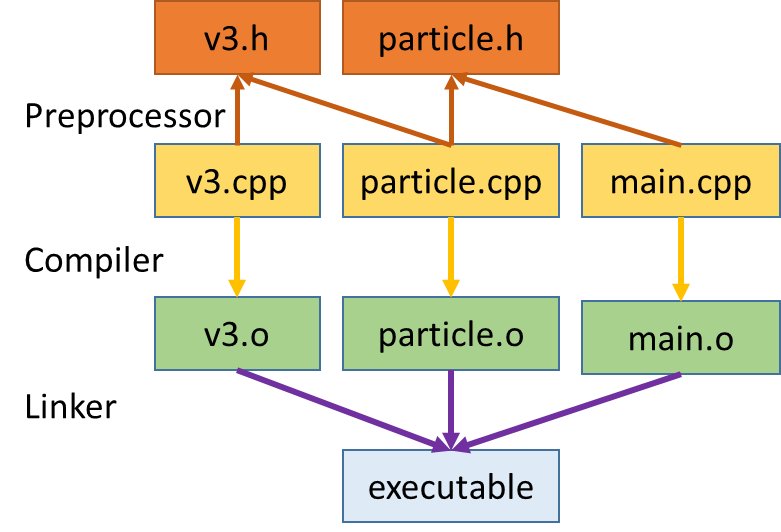
\includegraphics[scale=0.7]{../images/separate_compilation_linking.png}
\end{center}
Можно собрать всё сразу:
\begin{lstlisting}
g++ main.cpp particle.cpp v3.cpp
\end{lstlisting}
Либо можно собрать по частям:
\begin{lstlisting}
g++ -c main.cpp
g++ -c particle.cpp
g++ -c v3.cpp
g++ main.o particle.o v3.o
\end{lstlisting}

\subsection*{Виды библиотек:}
\begin{enumerate}
\item \textbf{header-only библиотеки:} Весь исходный код хранится в \texttt{.h} файле и подключается с помощью директивы \texttt{\#include} (очень просто подключить).
\item \textbf{Исходный код:} Библиотека поставляется в виде исходного кода (все \texttt{.h} и \texttt{.cpp} файлы). Для того чтобы использовать эту библиотеку, её нужно сначала скомпилировать, что может быть очень непросто для больших библиотек, так как процесс сборки может сильно отличаться на разных операционных системах и компиляторах.
\item \textbf{Статическая библиотека:} Библиотека поставляется в виде header-файлов(\texttt{.h}) и предварительно скомпилированных файлов библиотеки Расширение статических библиотек на linux: \texttt{.a} (archive). Расширение на windows: \texttt{.lib} (library). Эти библиотеки подключаются на этапе линковки. После линковки содержимое этих библиотек содержится в исполняемом файле. Такие библиотеки проще подключить к проекту, чем исходный код. Однако, вам обязательно иметь версию библиотеки, скомпилированную на такой же ОС и на таком же компиляторе, иначе она не подключится. Обратите внимание, что статические библиотеки обязательно должны иметь префикс \texttt{lib}. Например, если мы хотим получить библиотеку под названием \texttt{image}, то файл должен называться \texttt{libimage.a}.
\item \textbf{Динамическая библиотека:} Библиотека поставляется в виде header-файлов(\texttt{.h}) и предварительно скомпилированных файлов библиотеки Расширение динамических библиотек на linux: \texttt{.so} (от shared object). Расширение на windows: \texttt{.dll} (от dynamic link library)). Эти библиотеки подключаются на этапе \textit{выполнения программы}. Благодаря тому, что динамическая библиотека подключается на этапе выполнения, если несколько программ будут использовать одну и ту же библиотеку, то она будет загружаться в память лишь один раз.
\end{enumerate}

\subsection*{Задания:}
\begin{itemize}
\item \textbf{header:} В папке \texttt{1image/0header-only} лежит исходный код программы, которая использует класс \texttt{Image}. Это простой класс для работы с изображениями в формате \texttt{.ppm}. Скомпилируйте и запустите эту программу.
\item \textbf{Случайные отрезки:} Используйте этот класс, чтобы создать изображение, состоящее из 100 случайных отрезков случайного цвета. Для случайных чисел используйте функцию \texttt{rand()} из библиотеки \texttt{<cstdlib>}.
\item \textbf{Случайные прямоугольники:} Добавьте в этот класс метод \\
\texttt{void draw\_rectangle(const Vector2i\& bottomleft, const Vector2i\& torright, const Color\& color)}. Используйте этот метод, чтобы создать изображение, состоящее из 100 случайных прямоуголиников случайного цвета.
\item \textbf{Шум:} Добавьте в этот класс метод \texttt{void add\_noise(float probability)}, который будет добавлять шум на картинку: каждый пиксель с вероятностью \texttt{probability} должен поменять цвет на случайный. Протестируйте этот метод на картинках.
\item \textbf{Раздельная компиляция:} В папке \texttt{1image/1separate\_compilation} лежит тот же код, но разделённый на 2 файла исходного кода. Скомпилируйте эту программу с помощью \texttt{g++}.Добавьте функции \texttt{draw\_rectangle} и \texttt{add\_noise} из предыдущих заданий в этот проект.
\item \textbf{Статическая библиотека:} Чтобы создать свою статическую библиотеку вам нужно:
\begin{enumerate}
\item Создать объектный файл необходимого исходного файла.
\item Превратить объектный файл (или файлы) в библиотеку, используя утилиту \texttt{ar}:
\begin{verbatim}
ar rvs libimage.a image.o
\end{verbatim}
\item После этого файл \texttt{libimage.a} можно будет подключить к любому другому проекту примерно так:
\begin{verbatim}
g++ main.cpp -I<путь до header-файлов> -L<путь до libimage.a> -limage
\end{verbatim}
\end{enumerate}
В папке \texttt{1image/2static\_library} лежит исходный код программы. Вам нужно создать статическую библиотеку из файла \texttt{image.cpp} и поместить полученный файл в папку \texttt{image/lib}, а header-файл поместить в папку \texttt{image/include}. Затем вам нужно удалить файл \texttt{image.cpp} и собрать программу используя только статическую библиотеку (не забывайте про опции \texttt{-I}, \texttt{-L} и \texttt{-l}).
\item \textbf{Статическая библиотека 2:} В папке \texttt{1image/3static\_test} лежит проект с одной очень маленькой статической библиотекой (содержит 1 функцию). Вам нужно собрать этот проект и запустить исполняемый файл.
\item \textbf{Динамическая библиотека:} Чтобы создать динамическую библиотеку из файла исходного кода (\texttt{image.cpp}):
\begin{verbatim}
g++ -c -fPic image.cpp -o image.o
g++ -shared -o libimage.so image.o
\end{verbatim}
Чтобы скомпилировать код с подключением динамической библиотеки:
\begin{verbatim}
g++ -o main.exe main.cpp libimage.so
\end{verbatim}
или
\begin{verbatim}
g++ -o main.exe main.cpp -limage
\end{verbatim}
Но для этого понадобится добавить в переменную среды \texttt{LD\_LIBRARY\_PATH} путь до папки, содержащий библиотеку.
\begin{enumerate}
\item Создайте динамическую библиотеку и скомпилируйте саму программу с подключением динамической библиотеки
\item Проверьте чему равен размеры исполняемых файлов в случае подключения статической и динамической библиотеки.
\item Что будет происходить, если перенести файл динамической библиотеки в другую папку. Запустится ли исполняемый файл?
\end{enumerate}
\end{itemize}

\newpage
\section*{Часть 2: Библиотека SFML:}
Библиотека SFML (Simple and Fast Multimedia Library) - простая и быстрая библиотека для работы с мультимедиа. Кроссплатформенная (т. е. одна программа будет работать на операционных системах Linux, Windows и MacOS). Позволяет создавать окно, рисовать в 2D и 3D, проигрывать музыку и передавать информацию по сети. Для подключения библиотеки вам нужно скачать нужную версию с сайта: \href{https://www.sfml-dev.org/}{sfml-dev.org}.

\subsubsection*{Подключение вручную:}
Для подключения библиотеки вручную через опции \texttt{g++} нужно задать путь до папок \texttt{include/} и \texttt{lib/} и названия файлов библиотеки, используя опции \texttt{-I}, \texttt{-L} или \texttt{-l}. 
\begin{verbatim}
g++ .\main.cpp -I<путь до include> -L<путь до lib> -lsfml-graphics -lsfml-window -lsfml-system
\end{verbatim}
Например так:
\begin{verbatim}
g++ .\main.cpp -I./SFLL-2.5.1/include -L./SFLL-2.5.1/lib -lsfml-graphics -lsfml-window -lsfml-system
\end{verbatim}

\subsubsection*{\texttt{bash}-скрипт:} Так как постоянно прописывать в терминале сборку проекта может быть затруднительно, то можно положить весь процесс сборки в специальный \texttt{bash}-скрипт. \texttt{bash}-скрипт - это просто файл кода языка терминала linux. (Для windows есть аналогичные \texttt{bat}-скрипты) Пример можно посмотреть в \texttt{2sfml/1bash\_script}.

\subsubsection*{Makefile:} \texttt{make} -- это специальная утилита, предназначенная для упрощения сборки проекта. В \texttt{2sfml/3makefile} содержится пример проекта с make-файлом. Содержимое make-файла представляет собой просто набор целей и соответствующих команд оболочки \texttt{bash}. Откройте make-файл и просмотрите его содержимое. Чтобы скомпилировать его просто:
\begin{verbatim}
make <имя цели>
\end{verbatim}
либо просто
\begin{verbatim}
make
\end{verbatim}
(в этом случае \texttt{make} запустит процесс создания первой цели)

\subsection*{Задания:}
\begin{itemize}
\item \textbf{Сборка:} скомпилируйте и запустите проект. Используйте \texttt{bash}-скрипт или make-файл. Более подробно -- в папке \texttt{2sfml}.
\item \textbf{Движение по окружности:} Заставьте кружок двигаться по окружности. 
\item \textbf{Броуновское движение:} Создайте \texttt{n = 50} кругов, которые будут двигаться случайным образом (направление и величина движения должны задаваться случайным образом на каждом кадре).
\item \textbf{Задача n тел:} Создайте \texttt{n = 50} кругов, так, чтобы они притягивались друг к другу гравитационной силой. Начальные положения и скорости задайте случайным образом. Сила гравитации в двух измерениях обратно пропорциональна расстоянию между объектами.
$$
F \sim \frac{1}{R}
$$
\item \textbf{Задача N тел с массой} \\
Добавьте разную массу шарикам. При создании шарика масса должна задаваться случайным образом. Масса шарика должна быть пропорциональна площади (квадрату радиуса).
\item \textbf{Электрические заряды} \\
Смоделируйте взаимодействие заряженных частиц. Для этого нужно добавить поле в структуру \texttt{Ball}, которое будет определять величину заряда. Эта величина может быть как положительной, так и отрицательной. В начале работы программы заряд должен задаваться случайно. Заряды должны взаимодействовать по закону Кулона. Гравитацией можно пренебречь. Цвета зарядов должны быть различными (красный для положительного зарада и синий для отрицательного, интенсивность цвета - пропорциональна величине заряда).
\item \textbf{Нажатие мыши} \\
События нажатия мыши можно обработать с помощью следующего синтаксиса:
\begin{lstlisting}
if (event.type == sf::Event::MouseButtonPressed) 
{
    if (event.mouseButton.button == sf::Mouse::Right) 
    {
        std::cout << "the right button was pressed" << std::endl;
        std::cout << "mouse x: " << event.mouseButton.x << std::endl;
        std::cout << "mouse y: " << event.mouseButton.y << std::endl;
    }
}
\end{lstlisting}
Внутри цикла \texttt{while (window.pollEvent(event))}.\\
Видоизмените вашу программу так, чтобы при нажатии левой кнопки мыши в том месте, где находится мышь, создавался бы шарик со средними массой и средним положительным зарядом зарядом. При нажатии правой кнопки мыши должен создаваться шарик с очень большой  массой и очень большим положительным зарядом. При аналогичных нажатиях, но с зажатой клавишой Shift, должны создаваться отрицательные заряды.
\end{itemize}
\end{document}